\begin{table}[h]
\centering
\footnotesize
\renewcommand{\arraystretch}{1.2}
\begin{tabular}{|l|l|l|l|l|}
\hline
\textbf{Host} & \textbf{eth0} & \textbf{eth1} & \textbf{eth2} & \textbf{eth3} \\
\hline
h1a   & \texttt{fc00:0:1:a::1/64}    & N/A & N/A & N/A \\
h1b   & \texttt{fc00:0:1:b::1/64}    & N/A & N/A & N/A \\
h1c   & \texttt{fc00:0:1:c::1/64}    & N/A & N/A & N/A \\
h1d   & \texttt{fc00:0:1:d::1/64}    & N/A & N/A & N/A \\
\hline
as1ra & \texttt{fc00:0:1:ab::a/64}   & \texttt{fc00:0:1:ac::a/64}   & \texttt{fc00:0:1:ad::a/64}   & \texttt{fc00:0:1:a::a/64} \\
as1rb & \texttt{fc00:0:1:ab::b/64}   & \texttt{fc00:0:1:bc::b/64}   & \texttt{fc00:0:1:bd::b/64}   & \texttt{fc00:0:1:b::b/64} \\
as1rc & \texttt{fc00:0:1:ac::c/64}   & \texttt{fc00:0:1:bc::c/64}   & \texttt{fc00:0:1:cd::c/64}   & \texttt{fc00:0:1:c::c/64} \\
as1rd & \texttt{fc00:0:1:ad::d/64}   & \texttt{fc00:0:1:bd::d/64}   & \texttt{fc00:0:1:cd::d/64}   & \texttt{fc00:0:1:d::d/64} \\
\hline
\end{tabular}
\caption{IP-adressen per interface}
\label{tab:ip-adressen}
\end{table}

\begin{figure}[H]
    \centering
    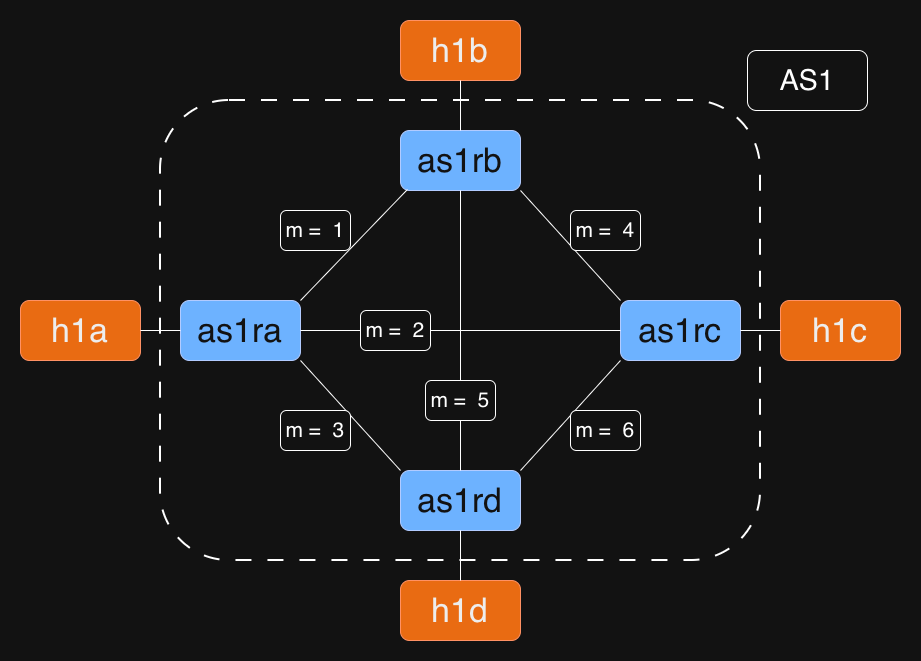
\includegraphics[width=1\textwidth]{traces/L4-4-1.drawio.png}
\end{figure}